\chapter{Introdução}
\label{cap:intro}
O uso de robôs baseados na fisiologia humana tem se tornado cada vez mais comum, entregando na maioria dos casos uma eficiência de produção superior à fornecida por trabalho humano. Em alguns casos, pode ser necessário o uso de robôs para a realização da tarefa especificada, como entrar em regiões de alto risco à saúde humana. Por este e outros muitos motivos, robôs cada vez mais robustos vêm sido desenvolvidos, com objetivos específicos e bem definidos. A principal vantagem de modelos humanoides sobre outros tipos terrestres, é a alta mobilidade em terrenos irregulares. No entanto, outras questões de caráter mais simples precisam ser resolvidas, como alcançar um nível de estabilidade na caminhada superior ou pelo menos parecido com o padrão humano.

Alguns trabalhos usam conceitos de física dinâmica para definirem o quão equilibrado o robô se encontra, em um determinado estado. A técnica mais abordada é o Zero Moment Point (ZMP)~\cite{Vukobratovic1968}, que diz que um robô está em equilíbrio quando a soma das forças e momentos resultantes sobre o corpo são anuladas pela força de reação aplicada em um ponto de pressão que se encontra sobre uma base formada por pontos em contato com o chão (SC), este ponto é denominado ZMP. Vale destacar que para o calculo do ZMP não é necessário considerar os limites da base de contato, podendo ele ser um ponto fictício~\cite{Vukobratovic2004}. Neste tipo de estratégia um controlador é implementado para gerar uma função de trajetória para o centro de massa ou uma cinemática de movimento para os atuadores, onde uma vez conhecida a posição dos pés de apoio, tem-se como objetivo garantir que o ZMP estará o máximo de tempo possível sobre a SC. Para realizar ajustes de equilíbrio, o controlador poderia também alterar as posições futuras dos pés no chão, além de modificar a cinemática ou função de trajetória do centro de massa (CoM)~\cite{Maximo2017}.

Outra abordagem que obteve bons resultados em ambiente simulado, é o controlador composto por redes neurais artificiais, como mostra (RNA)~\cite{Bin2017,Schulman2017}. Este método visa "ensinar" uma RNA a manipular os atuadores de um bípede humanoide, abstraindo a lógica de equilíbrio dos estados informados à rede, seguido da inferência de uma ação que possivelmente possa fornecer ao robô uma boa recompensa, com base na função objetivo estabelecida. Para isso, são simulados múltiplos casos com a RNA no controle das ações tomadas pelo robô, onde serão coletadas informações usadas para treinar o modelo. Os pares estado-ação que levarem o modelo a terem melhores resultados são recompensados, mapeando o conjunto universo dos estados em ações moldadas por uma função de recompensa.

\begin{figure}[H]
  \centering
  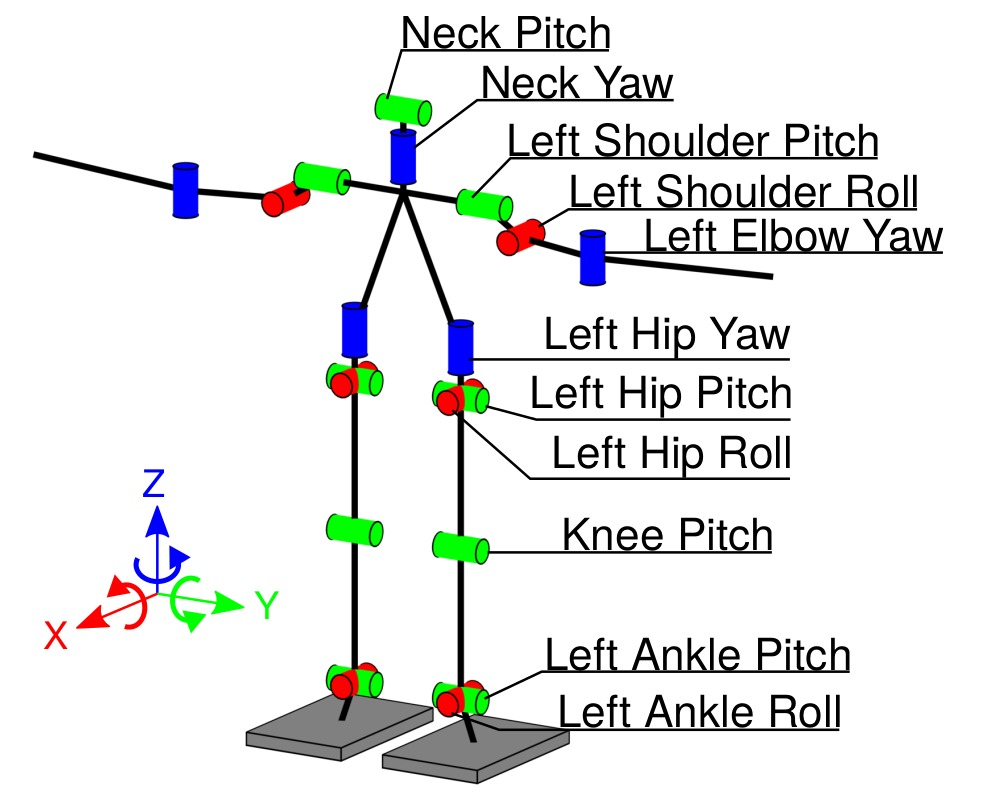
\includegraphics[width=0.7\textwidth]{./fig/fig10.jpeg}
  \caption{Arquitetura estrutural do robô ROBOTIS OP2 em relação ao sistema de coodenadas utilizado. Os nomes das juntas do lado direito seguem o mesmo padrão do lado esquerdo. Imagem retirada de ~\cite{Maximo2017}}
  \label{fig:sistema_coodenadas}
\end{figure}

O bípede humanoide utilizado neste trabalho possui uma arquitetura similar ao robô ROBOTIS OP2~\ref{fig:sistema_coodenadas}, com a diferença de não possuir os atuadores "Neck Pitch", "Neck Yaw", "Left Elbow Yaw" e "Right Elbow Yaw". O bípede possui 16 graus de liberdade (DoF) e é composto por atuadores com as configurações (stall torque, radial load limit, RPM) baseadas no servo-motor Dynamixel MX-28. Além disso, neste trabalhor usaremos o termo componentes horizontais para referenciar os eixos X e Y de um dado vetor, e componente vertical para referenciar o eixo Z.

